\documentclass[../thesis]{subfiles}

\begin{document}

\chapter{Architecture}
Characterization and development of sensor arrays presents a broad
range of research challenges, not least of which relate to data
organization. A \gls{LIMS} adequate to the needs of our example
application must provide

This chapter abstractly describes the constituent components
of the software framework we have built for collaborative design,
execution, and analysis of experiments. When describing each
element, we document some of the phases of our iterative design
process that led to these decisions.

\section{Physical architecture}
Ideally we would like for collaborating researchers at different
universities to be able to review each others' experiments in real
time, allowing for continuous feedback between investigators with
different areas of expertise.

\section{Network architecture}
% \begin{figure}
%   \includegraphics[width=\textwidth]{network-monolithic}
%   \caption{
%     Schematic of an example experimental apparatus for
%     characterizing an array of electrochemical gas sensors.
%     Inset: some commonly used stimulus waveforms for interrogating
%     electrochemical sensors.
%     \label{fig:EchemUseCase}
%   }
% \end{figure}

\subsection{Monolithic approach}


\subsection{Microservices}
As opposed to the conventional \gls{frontend}-\gls{backend} divide, some
developers have suggested an architecture for web applications based
on simple communicating modules termed \glspl{microservice}. In a
traditional monolithic architecture, programmers compose a complicated
application hierarchically, using one main module which calls library
functions from many subordinate components.  A microservice
architecture splits functionality into many independent programs which
communicate using ordinary network protocols, and modules are designed
to assume that their dependencies are completely separate programs
potentially running on other machines \cite{Micro14:online}.  This
approach promises better modularity than traditional web applications
since capabilities can be added and extended independently of one
another \cite{Balalaie2016}. Since all services expose their
functionality over a similar web \gls{API}, implementations are
decoupled from each other and internally have very different
architectures tailored to their special-purpose needs.  Services may
even be written in completely different programming languages. The
flexibility that this approach affords is a good fit with our desire
to adapt the framework to meet users' changing needs. Furthermore, a
microservice architecture lends itself naturally to a design where
capabilities and resources are distributed geographically, as is the
case with large, remotely collaborating groups of researchers. In some
cases microservice architectures also scale better as performance
demands on the system increase.

A schematic depicting the connections between some of our core
microservices can be found in figure \ref{fig:Microservices}.

\begin{figure}
  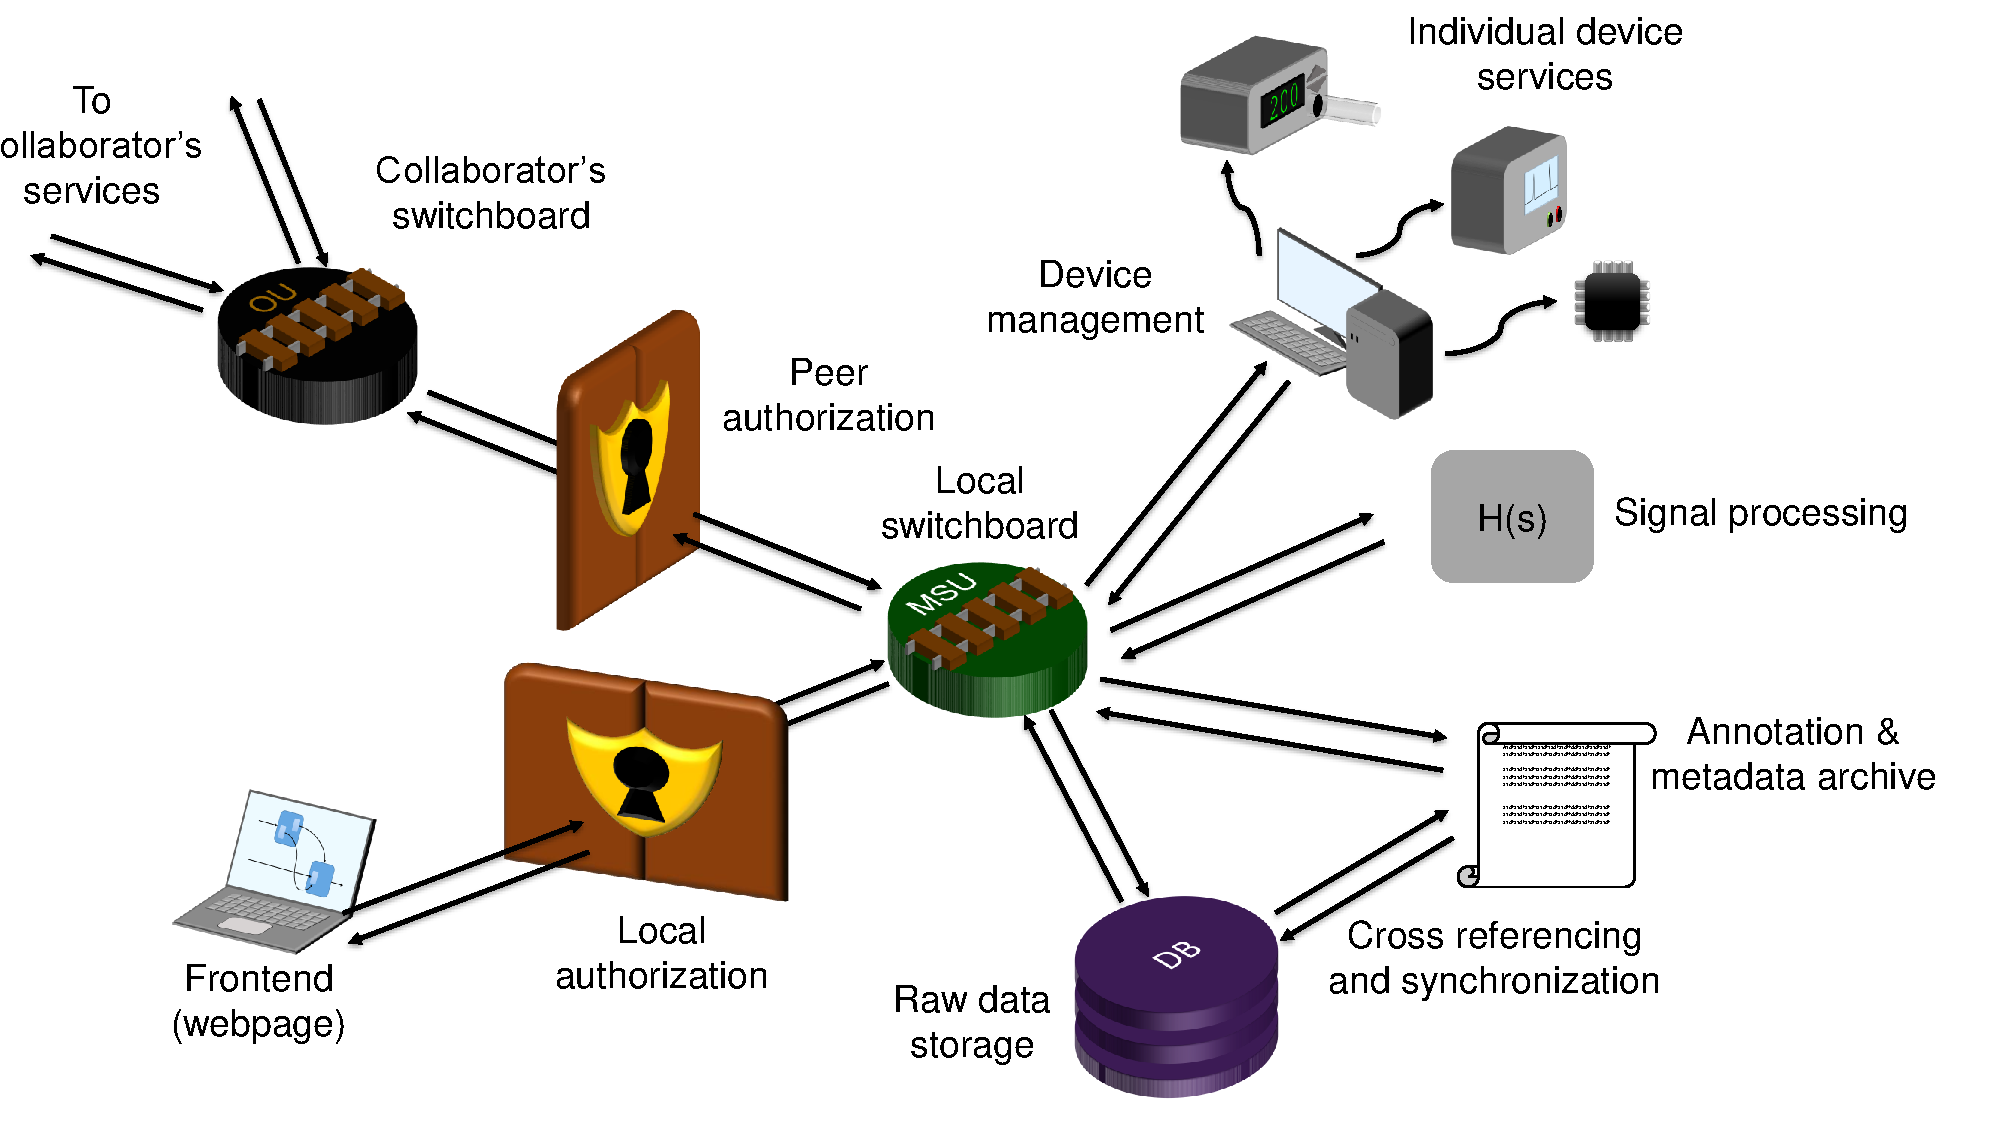
\includegraphics[width=\textwidth]{microservices}
  \caption{
    High-level interconnection between the critical microservices
    composing our final design.
    \label{fig:Microservices}
  }
\end{figure}

\subsection{Switchboard service}
Despite its internally distributed design, the web application must
present a primary gateway for user interaction. In our design this
role is taken by a microservice we refer to as a \gls{switchboard}

\section{Device control}
A core goal of our design is to enable researchers to incorporate
choreography of physical lab equipment into the executable workflows
they create. Interacting with the variety of commercial and custom
hardware found in a typical experimental lab requires a flexible
approach, given that computer control interfaces and data formats for
scientific equipment are heterogeneous and very poorly
standardized. This section describes an approach for building a
modular library of device drivers which integrate with the rest of the
system while providing users with tools for extension and
customization.

\subsection{Instrument manager}
The instrument manager is a microservice responsible for detecting
connected devices, determining the appropriate device driver for
communicating with them, and presenting a unified interface to the
switchboard.

\subsection{Interface API}

\subsection{Enumeration}

\subsection{Protocol composition}



\section{Data model}

\subsection{entity models}

\subsection{dataset tabulation}



\section{User experience}



\section{Security}



\end{document}
